\section{Methodology}
\subsection{Problem Formulation}
\label{sec:formulation}

\paragraph{World model formulation.}
We aim to learn a world model $\mathcal{W}_\theta$ that serves as a proxy for evaluating robotic policies.
Specifically, given a language instruction $l$, a current observation $o_t$, a history $h_t$, and a sequence of future actions $\mathbf{a}_t$, the model predicts the visual outcome $\hat{o}_{t+\Delta}$ and a task progress score $\hat{v}_{t+\Delta} \in [0,1]$ at horizon $\Delta$.
Essentially, $\mathcal{W}_\theta$ approximates the joint distribution of future visual dynamics and task completion: $(\hat{o}_{t+\Delta}, \hat{v}_{t+\Delta}) \sim \mathcal{W}_\theta(\cdot \mid o_t, \mathbf{a}_t, h_t, l)$.
To serve as a reliable evaluator, $\mathcal{W}_\theta$ must satisfy three properties:
(1) Action controllability: predictions must faithfully reflect the visual changes induced by the input actions;
(2) Spatiotemporal consistency: the model must preserve the spatial layout and consistency across long-horizon rollouts; and
(3) Discriminative task completion: generated future states must be semantically unambiguous to allow for accurate success detection.

\paragraph{Policy evaluation via imagination.}
We define an imagined rollout as a closed-loop interaction between a policy $\pi$ and the world model $\mathcal{W}_\theta$, yielding a generated trajectory $\tau = \{\hat{o}_0, \hat{o}_\Delta, \dots, \hat{o}_T\}$.
The policy's performance is evaluated by the imagined success rate $J = \frac{1}{N}\sum_{i=1}^N \mathcal{S}(\tau_i)$, where $\mathcal{S}(\cdot) \in \{0,1\}$ is a success indicator function that judges whether the generated outcome fulfills the task instruction.


\subsection{World Modeling via Discrete Diffusion}
\label{sec:architecture}

\subsubsection{Action Control via Unified Token Sequence}
\label{sec:action_tokenization}
To ensure action controllability, we integrate actions directly into a unified discrete token space, rather than treating them as auxiliary conditions. Specifically, we employ specialized tokenizers to map heterogeneous modalities into discrete codes: MAGVIT-v2~\cite{magvit-v2} for RGB observations, LLaDA~\cite{LLaDA} for language, and FAST~\cite{pertsch2025fast} for continuous action chunks $\mathbf{a}_t$. By serializing these codes into a single flattened sequence, the transformer can model the joint distribution of actions and observations.
Through self-attention, each visual token directly attends to action tokens, enabling fine-grained control at the token level. This allows that generated visual states accurately reflect the input actions.

% We employ specialized tokenizers to map each modality into a shared discrete latent space: MAGVIT-v2~\cite{magvit-v2} for RGB observations, the LLaDA tokenizer~\cite{LLaDA} for language instructions, and FAST~\cite{pertsch2025fast} for continuous action chunks $\mathbf{a}_t$.
% To unify these diverse representations, tokens from different modalities are mapped into a single index space via fixed offsets and serialized into a flattened sequence.
% Crucially, rather than processing actions as separate conditions, this joint sequence passes through a unified backbone with bidirectional attention.
% This design enables visual generation targets to attend directly to action tokens at every layer.
% We posit that such dense interaction treats actions as tokens of equal standing with visual observations, facilitating finer-grained modeling of action-causal dynamics and ensuring strict action controllability.



\begin{figure*}[t]
  \centering
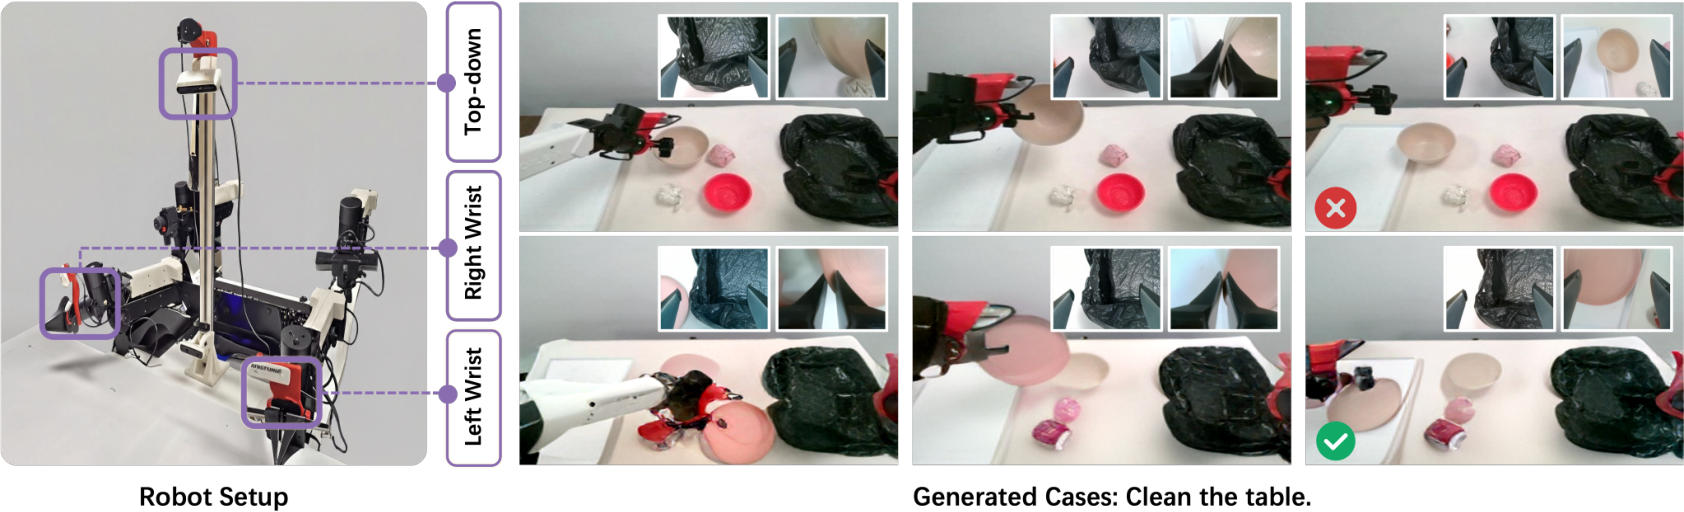
\includegraphics[width=0.95\textwidth]{figures/setup.pdf}
    \caption{\textbf{Real-world setup and rollout visualization.} \textbf{Left:} The bimanual AgileX platform equipped with three synchronized cameras. \textbf{Right:} Result of a failure and a success rollout generated for the \textit{Clean the Table} task; the insets in the top corners of each frame display the synchronized wrist views.}
  \label{fig:real_setup}
\end{figure*}

\subsubsection{Sparse Keyframe Memory for Spatiotemporal Consistency}
\label{sec:training_history}



To maintain spatiotemporal consistency, we employ a sparse keyframe memory. The memory is updated via a sliding window that samples the most recent $K$ frames at a fixed stride $\Delta$, aligned with the action chunk size. These sampled keyframes are tokenized and concatenated with other tokens described in Sec.~\ref{sec:action_tokenization}. To explicitly preserve temporal order within this sequence, we encode absolute frame indices as text tokens and prepend them to the corresponding history keyframes~\cite{guo2025seed1}.
To optimize computational efficiency, we encode history frames at a reduced resolution, utilizing only the fixed global view (e.g., top-down). This setup provides sufficient context for the model while significantly reducing token usage. In contrast, the current observation retains all views at full resolution to capture the fine-grained object interactions required for precise generation.

\subsubsection{Discrete Progress Token for Automatic Success Detection}
\label{sec:training_score}
Prior methods decouple success detection from visual generation, incurring additional overhead and potential inconsistency. Instead, our unified token space enables joint generation of visual outcomes and progress scores within a unified latent space, thereby aligning the predicted score with the generated content.
During training, we define task-specific milestones and prompt SEED-1.5VL~\cite{guo2025seed1} with few-shot examples to estimate task completion progress from visual observations (see Appendix~\ref{app:progress_grading} for details). The resulting scores are converted into discrete tokens (e.g., ``1.0'') and appended to the target sequence.
At inference, the generated text tokens are decoded into a numeric score $\hat{v}_{t+\Delta}$, enabling automatic computation of success rate for policy ranking.

\subsection{Joint Visual-and-Progress Denoising}
\label{sec:backbone}
We employ Masked Discrete Diffusion (MDD) to learn the transition distribution $p(\mathbf{y}_{t+\Delta} \mid \mathbf{c}_t)$, where the context $\mathbf{c}_t$ remains unmasked while the target suffix is partially masked for reconstruction. Specifically, during training, we sample a diffusion level $\lambda \sim \mathcal{U}(0,1)$ and corrupt the target via a mask-based forward process $\tilde{\mathbf{y}}_{t+\Delta} \sim q_\lambda(\tilde{\mathbf{y}} \mid \mathbf{y}_{t+\Delta})$. The model is then optimized to reconstruct the clean tokens at the masked indices $\Omega_\lambda = \{j \mid \tilde y_j = \texttt{[MASK]}\}$ by minimizing the following weighted objective:
\begin{equation}
\mathcal{L}_{\text{WM}}
=
\mathbb{E}_{\tau,\lambda,\tilde{\mathbf{y}}}
\Bigg[
-\frac{1}{m(\lambda)}
\sum_{j\in\Omega_\lambda}
w_j \log p_\theta\!\left(
y_j \mid
\mathbf{c}_t,\tilde{\mathbf{y}}_{t+\Delta},\lambda
\right)
\Bigg],
\label{eq:loss_total}
\end{equation}
where $m(\lambda)$ denotes the masking probability at level $\lambda$, and $w_j$ serves as a modality-specific rebalancing weight. At inference, we use iterative parallel decoding to sample $\mathbf{y}_{t+\Delta}$ conditioned on the unified context $\mathbf{c}_t$. This process simultaneously generates the future visual state and its progress score.
